\chapter{Solução proposta}\label{chap:solucao}

Visto que o \cddl somente exporta à camada de aplicação, eventos de leitura de dados de contexto.
Significando que, dentre todos os objetos do tipo \sensordata criados no \stwopa, apenas aqueles com atributo ``\texttt{action}'' assumindo valor ``\texttt{READ}'' eram propagados ao \qocevaluator no \cddl podendo assim serem percebidos pela aplicação (vide \autoref{subsub:s2pa}).

Este fato implica em algumas limitações no desenvolvimento de aplicações.
Imagine um cenário onde uma aplicação necessite de certos dados providos por um \smartobj---alocando recursos computacionais para processá-los.
Em uma eventual desconexão com o \smartobj, o fluxo de dados do sensor cessaria de ser entregue à aplicação, contudo, nenhum fluxo ou notificação do evento de desconexão seria entregue.
A aplicação não poderia decidir se o interrompimento do fluxo de dados se deu, devido a uma mudança na latência do envio de dados por parte do sensor ou por uma desconexão, não podendo então decidir sobre a necessidade da desalocação de recursos.

Esta limitação do \cddl dificultava ainda o desenvolvimento de aplicações que interagem com \smartobjs no ambiente por outros meios além de conexões.
É o caso de aplicações de localização \textit{indoor} baseadas em \beacons \bluetooth, onde os \beacons são dispostos no interior de ambientes físicos e permanecem realizando \broadcast de sua presença.
Os dispositivos móveis não realizam tentativas de conexão, apenas percebem a presença destes \smartobjs e utilizam a intensidade do sinal capturado no momento.

O trabalho em questão tem como objetivo a implementação do mecanismo que propaga os eventos de descoberta, conexão e desconexão que ocorrem no \stwopa do \mhub até a camada de aplicação do \cddl, de forma que os desenvolvedores possam projetar aplicações que se adaptem a tais eventos.

Vale ressaltar que a implementação também deve permitir que estes eventos possam estar disponíveis para outras aplicações que estejam interessadas, utilizando para isso o \mqtt.
Ou seja---caso configurado desta forma---uma aplicação \mhubcddl pode mudar seu comportamento baseado em eventos que foram disparados a partir de interações entre \smartobjs e \smartphones remotos.

\section{Requisitos de \software}

\subsection*{Requisitos funcionais}

Os requisitos funcionais definidos para a solução são:

\begin{alineas}
	\item notificação de eventos de descoberta, conexão e desconexão de \smartobjs para a camada de aplicação do \software;

	\item separação dos fluxos de eventos, provendo uma \api que permita a aplicação registrar interesse em cada tipo de evento individualmente;

	\item permitir que estes eventos possam estar acessíveis tanto para a aplicação que os gera, quanto para aplicações remotas que registrem interesse em interações de outros \smartphones com \smartobjs;

	\item fornecer uma \api assíncrona para o recebimento de cada notificação dos eventos desejados.
\end{alineas}

\section{Implementação}

\subsection{Propagação de eventos do \stwopa para o \cddl}

Como descrito na \autoref{subsub:s2pa}, o \mhub encapsula todos os eventos em objetos do tipo \sensordata, estes objetos devem então ser propagados para o \cddl.
O \stwopa comunica-se com o \cddl através do componente \qocevaluator, como pode ser observado na \autoref{fig:mhub-cdll-architecture}~\cite{gomes:2017}.

A comunicação entre os componentes é feita através da biblioteca \eventbus\footnote{\url{http://greenrobot.org/eventbus/}}.
O \eventbus é uma biblioteca de eventos de código livre escrita em Java para a plataforma \android utilizando o padrão \pubsub, fornecendo um mecanismo central de comunicação simplificando a interação entre componentes da aplicação.

O \stwopa foi modificado então para publicar cada \sensordata no \eventbus, enquanto o \qocevaluator registra interesse em receber objetos do tipo \sensordata publicados no \eventbus.
O que efetivamente transfere todos os eventos gerados pelo \stwopa ao \cddl.

\subsection{Separação dos fluxos de eventos}

Como todos os dados publicados pelo \cddl são do tipo \msg, decidiu-se manter este padrão, de forma a manter a retrocompatibilidade e assim continuar suportando as aplicações antigas.
Ao invés de utilizar a estratégia adotada pelo \mhub (utilizar um atributo que identifica que tipo de evento o objeto está representando), adotou-se uma estratégia baseada em orientação a objetos.
Foram criadas quatro novas classes que herdam os atributos de \msg, são elas:

\begin{alineas}
	\item \objfoundmsg: Para os eventos de descoberta;
	\item \objconnectedmsg: Para os eventos de conexão;
	\item \objdisconnectedmsg: Para os eventos de desconexão;
	\item \sensordatamsg: Para eventos de leitura de dados.
\end{alineas}

Com esta abordagem é possível utilizar a \api e métodos existentes, valendo-se do mecanismo de polimorfismo da orientação a objetos.
Ao receber um \sensordata, o \qocevaluator faz o seguinte: identifica, utilizando o atributo \texttt{action}, que tipo de evento ele representa; instancia um objeto de um dos tipos descritos anteriormente; e o publica no \broker \mqtt como um objeto do tipo \msg.


\subsection{Definição da estrutura de tópicos}

De forma a gerar fluxos diferentes para cada evento, e permitir consultas mais expressivas, o \qocevaluator deve publicar cada mensagem gerada em um tópico específico, de acordo com o tipo de evento que este representa.

A estrutura de tópicos proposta para publicação de eventos de descoberta, conexão e desconexão segue o seguinte padrão:
\[
	\underbrace{\bm{\mathsf{domain}}\vphantom{p}}_{\text{\textsf{identificador do \cddl}}}
	\bm{/}
	\underbrace{\bm{\mathsf{clientId}}\vphantom{p}}_{\text{\textsf{identificador do cliente}}}
	\bm{/}
	\underbrace{\bm{\mathsf{eventTopic}}}_{\text{\textsf{identificador do tipo de evento}}}
\]
Onde:

\begin{alineas}
	\item \emph{domain}: É um prefixo que compõe o primeiro nível de todos os tópicos gerados pelo \cddl, isto permite que seja possível identificar as mensagens publicadas no contexto do \middleware mesmo que um \broker público seja utilizado (\textit{e.g.}, realizando uma inscrição no tópico \texttt{domain/\#}).

	\item \emph{clientId}: É um identificador da aplicação cliente que gerou tal mensagem. Este valor é informado pelo desenvolvedor ao iniciar o \cddl;

	\item \emph{eventTopic}: Identificador único para cada tipo de evento, ou seja, para os eventos de descoberta, conexão e desconexão:
	\begin{alineas}
		\item \texttt{object\_found\_topic}: Para os eventos de descoberta;
		\item \texttt{object\_connected\_topic}: Para os eventos de conexão;
		\item \texttt{object\_disconnected\_topic}: Para os eventos de desconexão.
	\end{alineas}
\end{alineas}


A fim de se inscrever em eventos gerados por outras aplicações \mhubcddl, faz-se uso dos caracteres coringa do \mqtt descritos na \autoref{subsec:mqtt-topics}. Fazendo com que a aplicação se inscreva em tópicos com o seguinte padrão: \texttt{domain/+/eventTopic}.

%Caso a aplicação não possua o requisito de compartilhar os eventos gerados por ela com outras aplicações, pode-se utilizar o \ubroker embarcado disponível na plataforma \mhubcddl.

A \autoref{fig:solution-sequence} apresenta o diagrama de sequência do funcionamento da solução proposta. Ilustrando, neste caso, o processo de notificação de eventos de descoberta.

\begin{figure}[htb]
	\centering
	\caption{Diagrama de sequência do mecanismo implementado}
	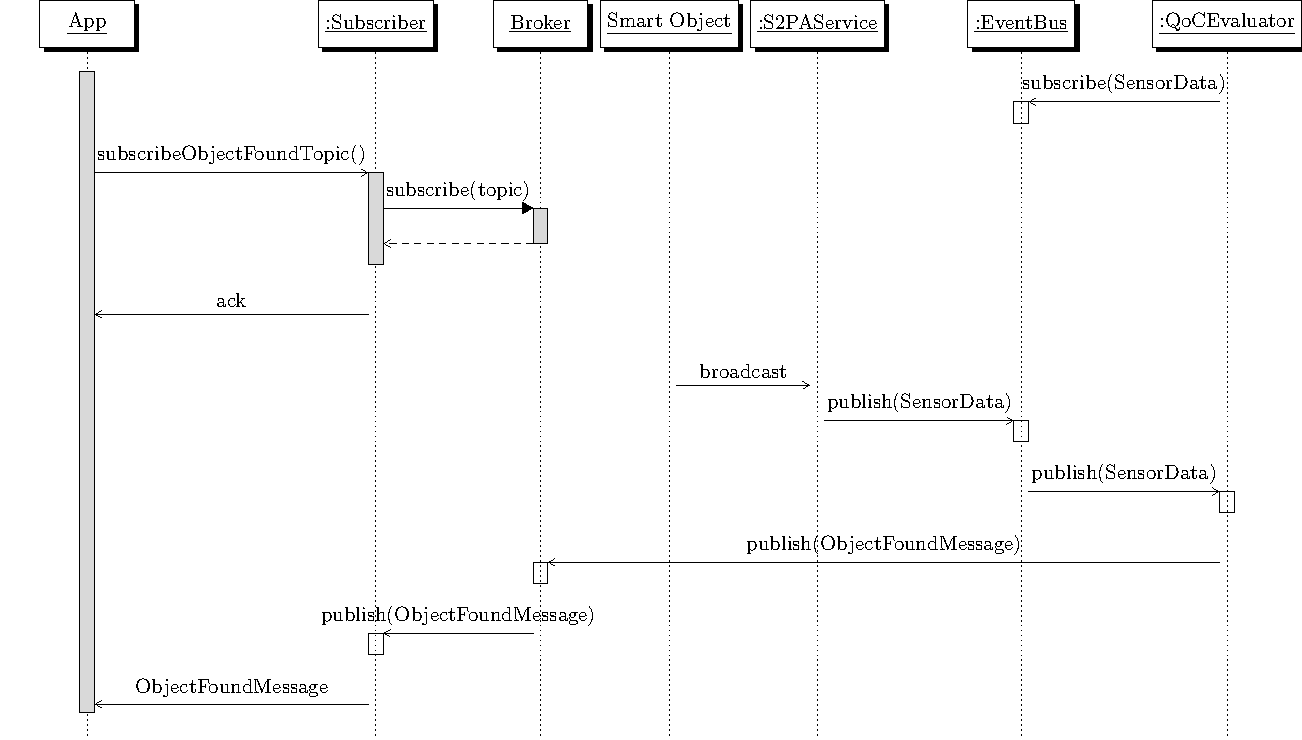
\includegraphics[width=0.95\textwidth]{img/solution-sequence.pdf}
	\fonte{\autoriapropria}
	\label{fig:solution-sequence}
\end{figure}

\subsection{Modelo de programação}

Foram então adicionados métodos à interface \texttt{Subscriber} que permitem que a aplicação registre interesse em cada tipo de evento gerado através de interações entre \smartobjs e o próprio dispositivo móvel em que executa, e também métodos que permitem que a aplicação receba eventos gerados por outras aplicações. Estes métodos inscrevem a aplicação no tópico \mqtt específico, e estão descritos adiante:

\begin{alineas}
	\item \texttt{subscribeObjectFoundTopic()}:
	\begin{alineas}
		\item Inscreve a aplicação no tópico \texttt{domain/userId/object\_found\_topic}, fazendo com que ela receba os eventos de descoberta de \smartobjs.
	\end{alineas}

	\item \texttt{subscribeObjectConnectedTopic()}:
	\begin{alineas}
		\item Inscreve a aplicação no tópico \texttt{domain/userId/object\_connected\_topic}, fazendo com que ela receba os eventos de conexão de \smartobjs.
	\end{alineas}

	\item \texttt{subscribeObjectDisconnectedTopic()}:
	\begin{alineas}
		\item Inscreve a aplicação no tópico \texttt{domain/userId/object\_disconnected\_topic}, fazendo com que ela receba os eventos de desconexão de \smartobjs.
	\end{alineas}
\end{alineas}


Aplicações que estão interessadas em certo tipo de serviço receberão uma instância de \msg a cada evento gerado.
Como ela é superclasse das anteriores,
caso a aplicação deseje diferenciar qual tipo de evento o objeto \msg que ela recebeu representa, é possível verificar em tempo de execução se determinado objeto é instância das classes mais especializadas, como é mostrado no \autoref{lst:polymorphism}.

\lstinputlisting[float=htb, label=lst:polymorphism, caption=Uso das classes mais especializadas em conjunto com a \api existente]{code/Polymorphism.java}

Nas linhas 1 e 2 uma instância de \texttt{Subscriber} é criada e uma conexão com um \broker estabelecida.
Nas linhas 3 e 4, a aplicação registra interesse em eventos de conexão e desconexão.
Como foi realizado a inscrição em múltiplos tópicos com um único \sub, todas as mensagens serão entregues em um mesmo \textit{listener}, que é definido na linha 6.
Nas linhas 9 e 11, a aplicação determina se o objeto que recebeu é instância de \objconnectedmsg ou \objdisconnectedmsg.
Desta forma pode escolher o comportamento mais adequado para cada evento.

